%%%%%%%%%%%%%%%%%%%%%%%%%%%%% Define Article %%%%%%%%%%%%%%%%%%%%%%%%%%%%%%%%%%
\documentclass{article}
%%%%%%%%%%%%%%%%%%%%%%%%%%%%%%%%%%%%%%%%%%%%%%%%%%%%%%%%%%%%%%%%%%%%%%%%%%%%%%%

%%%%%%%%%%%%%%%%%%%%%%%%%%%%% Using Packages %%%%%%%%%%%%%%%%%%%%%%%%%%%%%%%%%%
\usepackage[utf8]{inputenc}
\usepackage{float}
\usepackage{geometry}
\usepackage{amssymb}
\usepackage{amsthm}
\usepackage{amsmath}
\usepackage{graphicx}
\usepackage[breaklinks]{hyperref}
\usepackage{listings}
\usepackage{pdfpages}
\usepackage{comment}
\usepackage{fancyhdr}
\usepackage[english]{babel}
\usepackage{empheq}
\usepackage{mdframed}
\usepackage{booktabs}
\usepackage{lipsum}
\usepackage{color}
\usepackage{psfrag}
\usepackage{pgfplots}
\usepackage{bm}
\usepackage{wrapfig}
\usepackage{bookmark}
\usepackage{titlesec}
\usepackage{hyperref}
\usepackage{parskip}
\usepackage{capt-of}
\usepackage{subcaption}
\usepackage{tikz}
\usetikzlibrary{automata, positioning}
%%%%%%%%%%%%%%%%%%%%%%%%%%%%%%%%%%%%%%%%%%%%%%%%%%%%%%%%%%%%%%%%%%%%%%%%%%%%%%%

% Other Settings
% Other Settings
\hypersetup{
    colorlinks = true,
    linkcolor = black,
    urlcolor = blue,
}
\urlstyle{same}

%%%%%%%%%%%%%%%%%%%%%%%%%% Page Setting %%%%%%%%%%%%%%%%%%%%%%%%%%%%%%%%%%%%%%%
\geometry{a4paper}
\pagestyle{fancy}

%%%%%%%%%%%%%%%%%%%%%%%%%% Code Environment Setting %%%%%%%%%%%%%%%%%%%%%%%%%%%%%%%%%%%%%%%
\definecolor{codebackground}{rgb}{0.95,0.95,0.95}
\definecolor{codegray}{rgb}{0.5,0.5,0.5}
\definecolor{codepurple}{rgb}{0.58,0,0.82}
\definecolor{codeblue}{rgb}{0.13,0.29,0.53}

\lstset{
    language=Matlab,
    basicstyle=\ttfamily\small,
    backgroundcolor=\color{codebackground},
    commentstyle=\color{deepGreen},
    keywordstyle=\color{blue}, 
    stringstyle=\color{red},  
    numbers=left,
    numberstyle=\tiny\color{codegray},
    rulecolor=\color{black},
    frame=single,
    showstringspaces=false,
    breaklines=true,
    tabsize=4,
    captionpos=b,
    xleftmargin=10pt
}

%%%%%%%%%%%%%%%%%%%%%%%%%% Define some useful colors %%%%%%%%%%%%%%%%%%%%%%%%%%
\definecolor{ocre}{RGB}{243,102,25}
\definecolor{mygray}{RGB}{243,243,244}
\definecolor{deepGreen}{RGB}{26,111,0}
\definecolor{shallowGreen}{RGB}{235,255,255}
\definecolor{deepBlue}{RGB}{61,124,222}
\definecolor{shallowBlue}{RGB}{235,249,255}
%%%%%%%%%%%%%%%%%%%%%%%%%%%%%%%%%%%%%%%%%%%%%%%%%%%%%%%%%%%%%%%%%%%%%%%%%%%%%%%

%%%%%%%%%%%%%%%%%%%%%%%%%% Define an orangebox command %%%%%%%%%%%%%%%%%%%%%%%%
\newcommand\orangebox[1]{\fcolorbox{ocre}{mygray}{\hspace{1em}#1\hspace{1em}}}
%%%%%%%%%%%%%%%%%%%%%%%%%%%%%%%%%%%%%%%%%%%%%%%%%%%%%%%%%%%%%%%%%%%%%%%%%%%%%%%

%%%%%%%%%%%%%%%%%%%%%%%%%%%% English Environments %%%%%%%%%%%%%%%%%%%%%%%%%%%%%
\newtheoremstyle{mytheoremstyle}{3pt}{3pt}{\normalfont}{0cm}{\rmfamily\bfseries}{}{1em}{{\color{black}\thmname{#1}~\thmnumber{#2}}\thmnote{\,--\,#3}}
\newtheoremstyle{myproblemstyle}{3pt}{3pt}{\normalfont}{0cm}{\rmfamily\bfseries}{}{1em}{{\color{black}\thmname{#1}~\thmnumber{#2}}\thmnote{\,--\,#3}}
\theoremstyle{mytheoremstyle}
\newmdtheoremenv[linewidth=1pt,backgroundcolor=shallowGreen,linecolor=deepGreen,leftmargin=0pt,innerleftmargin=20pt,innerrightmargin=20pt,]{theorem}{Theorem}[section]
\theoremstyle{mytheoremstyle}
\newmdtheoremenv[linewidth=1pt,backgroundcolor=shallowBlue,linecolor=deepBlue,leftmargin=0pt,innerleftmargin=20pt,innerrightmargin=20pt,]{definition}{Definition}[section]
\theoremstyle{myproblemstyle}
\newmdtheoremenv[linecolor=black,leftmargin=0pt,innerleftmargin=10pt,innerrightmargin=10pt,]{problem}{Problem}[section]
%%%%%%%%%%%%%%%%%%%%%%%%%%%%%%%%%%%%%%%%%%%%%%%%%%%%%%%%%%%%%%%%%%%%%%%%%%%%%%%

%%%%%%%%%%%%%%%%%%%%%%%%%%%%%%% Plotting Settings %%%%%%%%%%%%%%%%%%%%%%%%%%%%%
% \usepgfplotslibrary{colorbrewer}
% \pgfplotsset{width=8cm,compat=1.9}
%%%%%%%%%%%%%%%%%%%%%%%%%%%%%%%%%%%%%%%%%%%%%%%%%%%%%%%%%%%%%%%%%%%%%%%%%%%%%%%

%%%%%%%%%%%%%%%%%%%%%%%%%%%%%%% Title & Author %%%%%%%%%%%%%%%%%%%%%%%%%%%%%%%%
\title{Statistics and Inferencing\\ Activity 02}
\author{Ali Muhammad Asad\\ aa07190}
\date{} %Leave uncommented if u want automatic date which is done through maketitle, else u can uncomment this and type anything else u want over here - not necessary to enter a date over here
%%%%%%%%%%%%%%%%%%%%%%%%%%%%%%%%%%%%%%%%%%%%%%%%%%%%%%%%%%%%%%%%%%%%%%%%%%%%%%%

\pgfplotsset{compat=1.18}

\begin{document}
\maketitle

The purpose of this activity is to:
\begin{enumerate}
    \item Consider a distribution. Generate data samples from the distribution using appropriate MATLAB function.
    \item Visualize the data using histogram,
    \item Normalize the histogram and compare it with the probability density function of considered distribution.
\end{enumerate}

Modify the code given for Gamma Distribution and repeat for the following:
\begin{enumerate}
    \item[(a)] Uniform Distribution
    \item[(b)] Gaussian Distribution
    \item[(c)] Exponential Distribution
    \item[(d)] Rayleigh Distribution   
\end{enumerate}

\newpage
\subsection*{Gamma Distribution}

\textbf{MATLAB Code:}
\begin{lstlisting}[caption={Gamma Distribution},label={Gamma}]
>> alpha = 2; beta = 0.5;
>> xmax = 20; x = 0:0.01:xmax;
>> fx = beta^alpha*x.^(alpha-1).*exp(-beta*x)/gamma(alpha);
>> k = alpha; theta = 1/beta;
>> DATA = gamrnd(k, theta, 1, 5000);
>> BINS = 30;
>> [COUNTS,EDGES] = histcounts(DATA,BINS);
>> Ediff = diff(EDGES);
>> WIDTH = Ediff(1);
>> AREA = sum(COUNTS)*WIDTH;
>> figure; bar(EDGES(1:end-1),COUNTS/AREA);
>> hold on; plot(x, fx, 'k-', 'linewidth', 2)
\end{lstlisting}

\begin{figure}[htbp]
    \begin{subfigure}[b]{0.5\textwidth}
        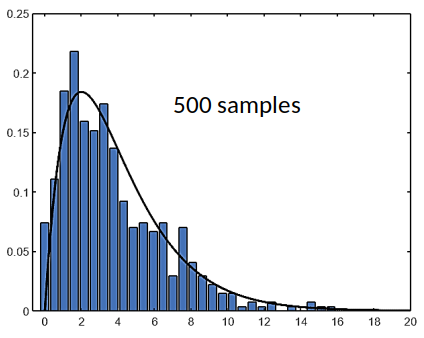
\includegraphics[width=\linewidth]{gamma_5.png}
        \caption{Gamma Distribution with 500 Data Points}
    \end{subfigure}
    \begin{subfigure}[b]{0.5\textwidth}
        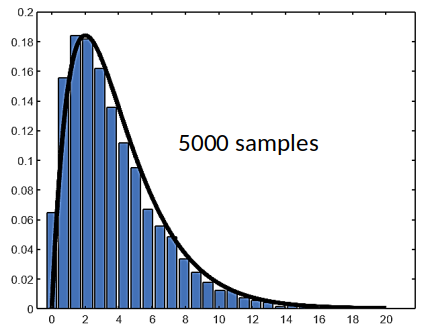
\includegraphics[width=\linewidth]{gamma_5k.png}
        \caption{Gamma Distribution with 5000 Data Points}        
    \end{subfigure}
\end{figure}
The Gamma Distribution is a continuous probability distribution that is defined by two parameters: the shape parameter $k$ or $\alpha$, and the scale parameter $\theta$ where $ \theta = \frac{1}{\beta} $. It's often used to model the time until an event occurs, such as the time until a radioactive particle decays or the time until a customer arrives at a service center.

The shape of the Gamma Distribution can vary widely depending on the values of the shape and scale parameters. It can be right-skewed, left-skewed, or symmetrical. Here we can see that the Gamma Distribution is right-skewed, with a peak around 2, which was equal to the shape parameter $\alpha$.

\newpage
\subsection*{Uniform Distribution}

\textbf{MATLAB Code:}
\begin{lstlisting}[caption={Uniform Disttribution},label={Uniform}]
>> a = 2; b = 2; %Minimum and Maximum Values
>> samples = 500; %Change samples to 5000 for 5000 data points
>> DATA = a + (b - a)*rand(1, samples);
>> BINS = 30;
>> [COUNTS,EDGES] = histcounts(DATA,BINS);
>> Ediff = diff(EDGES);
>> WIDTH = Ediff(1);
>> AREA = sum(COUNTS)*WIDTH;
>> figure; bar(EDGES(1:end-1),COUNTS/AREA);
>> title('UNIFORM DISTRIBUTION (500 Data Points)'); grid on;
\end{lstlisting}

\begin{figure}[htbp]
    \begin{subfigure}[b]{0.5\textwidth}
        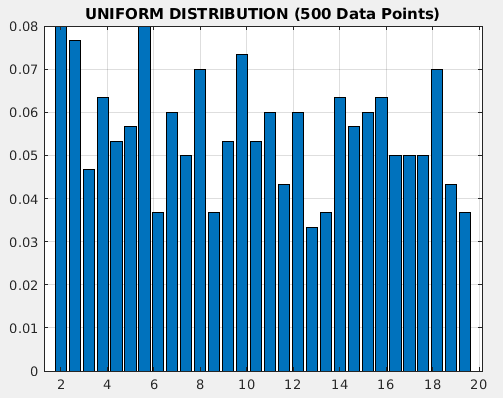
\includegraphics[width=\linewidth]{uniform_5.png}
    \end{subfigure}
    \begin{subfigure}[b]{0.5\textwidth}
        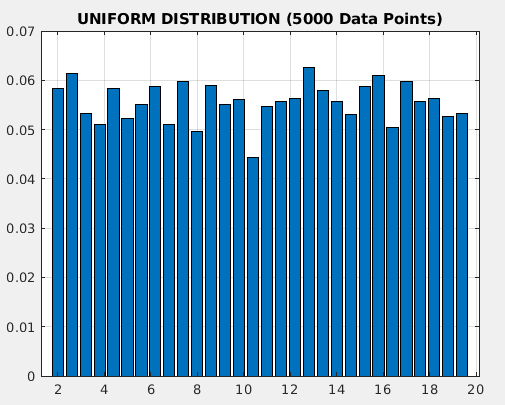
\includegraphics[width=\linewidth]{uniform_5k.png}    
    \end{subfigure}
\end{figure}

The Uniform Distribution is a continuous probability distribution that is characterized by a constant probability density function (PDF) over a specified interval. It's defined by two parameters: the minimum value ($a$) and the maximum value ($b$). The PDF is flat within this interval and zero outside of it. The Uniform Distribution becomes more and more uniform as we increase the data samples, as can be clearly seen from the above figures which draws a comparison between the Uniform Distribution with 500 and 5000 data points.

In comparison with the Gamma Distribution, we can clearly see that the Uniform Distribution approaches a constant shape between its parameters $a$ and $b$ as the number of data points increases, whereas the Gamma Distribution approaches a peak value, and its shape can vary depending on its parameters. \\ The Uniform Distribution has a fixed range [a, b], which means all values within this range have equal probabilities. In contrast, the Gamma Distribution can have a variable range and is not constrained to a specific interval. 

\newpage
\subsection*{Gaussian (Normal) Distribution}

\textbf{MATLAB Code:}
\begin{lstlisting}[caption={Gaussian (Normal) Distribution},label={Gaussian}]
>> mu = 2.5; sigma = 1.2; %Mean and Standard Deviation
>> DATA = mu + sigma * randn(1, 500); %Change value of randn from 500 to 5000 for data points
>> BINS = 30; 
>> [COUNTS,EDGES] = histcounts(DATA,BINS); 
>> Ediff=diff(EDGES);
>> WIDTH=Ediff(1); AREA = sum(COUNTS)*WIDTH;
>> figure; bar(EDGES(1:end-1),COUNTS/AREA);
>> title('Gaussian(Normal) Distribution (500 Data Points)');
>> grid on;
\end{lstlisting}

\begin{figure}[htbp]
    \begin{subfigure}[b]{0.5\textwidth}
        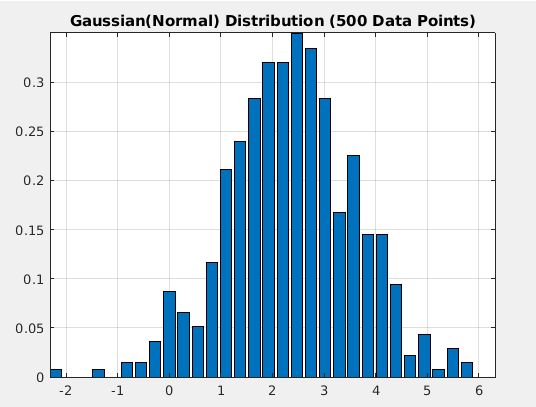
\includegraphics[width=\linewidth]{gauss_5.png}
    \end{subfigure}
    \begin{subfigure}[b]{0.5\textwidth}
        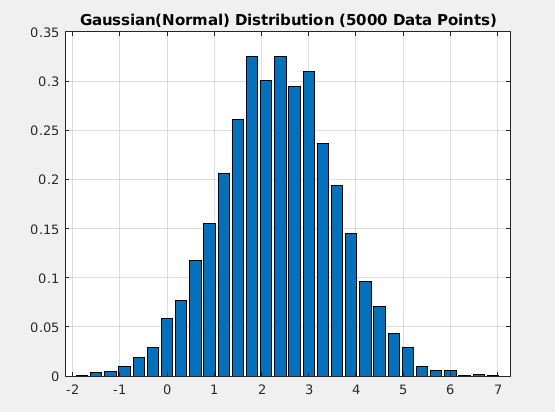
\includegraphics[width=\linewidth]{gauss_5k.png}    
    \end{subfigure}
\end{figure}

The Gaussian Distribution is a continuous probability distribution characterized by a bell-shaped curve. It's defined by two parameters: the mean $\mu$ and the standard deviation $\sigma$. It's widely used to model data that tends to cluster around a central value with symmetrically decreasing probabilities as values move away from the mean - so the peak of the distribution occurs at its mean (expected) value. Unlike the Gamma Distribution which is not symmetrical and can take on various shapes or be skewed. 

In addition, the shape of the Gaussian Distribution is primarily determined by the mean and standard deviation parameters. Changing these parameters shifts or scales the bell-shaped curve.


\newpage
\subsection*{Exponential Distribution}

\textbf{MATLAB Code:}
\begin{lstlisting}[caption={Exponential Distribution},label={Exponential}]
>> lambda = 0.5; %Rate Parameter
>> DATA = exprnd(1/lambda, 1, 500); %Change the value from 500 to 5000 for 5000 data points
>> BINS = 30; 
>> [COUNTS, EDGES] = histcounts(DATA,BINS); 
>> Ediff=diff(EDGES); 
>> WIDTH=Ediff(1);
>> AREA= sum(COUNTS)*WIDTH;
>> figure; bar(EDGES(1:end-1),COUNTS/AREA);
>> title('Exponential Distribution (500 Data Points)'); 
>> grid on;
\end{lstlisting}

\begin{figure}[htbp]
    \begin{subfigure}[b]{0.5\textwidth}
        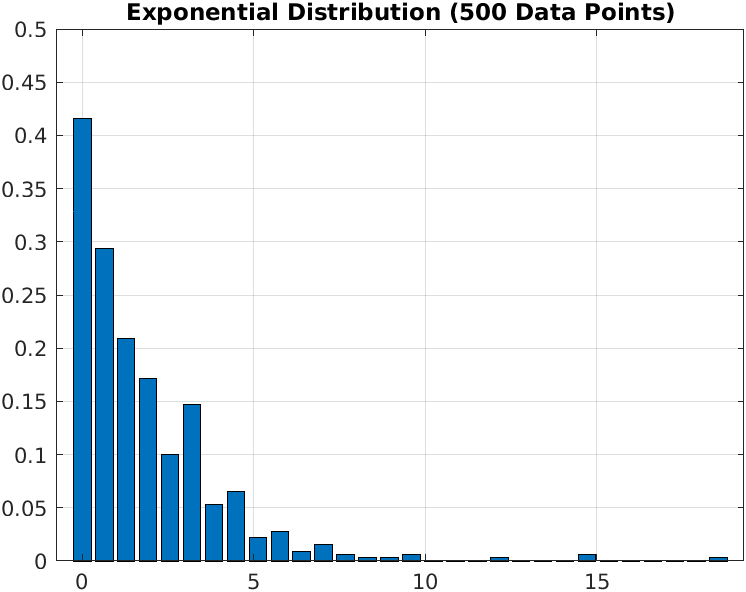
\includegraphics[width=\linewidth]{exp_5.png}
    \end{subfigure}
    \begin{subfigure}[b]{0.5\textwidth}
        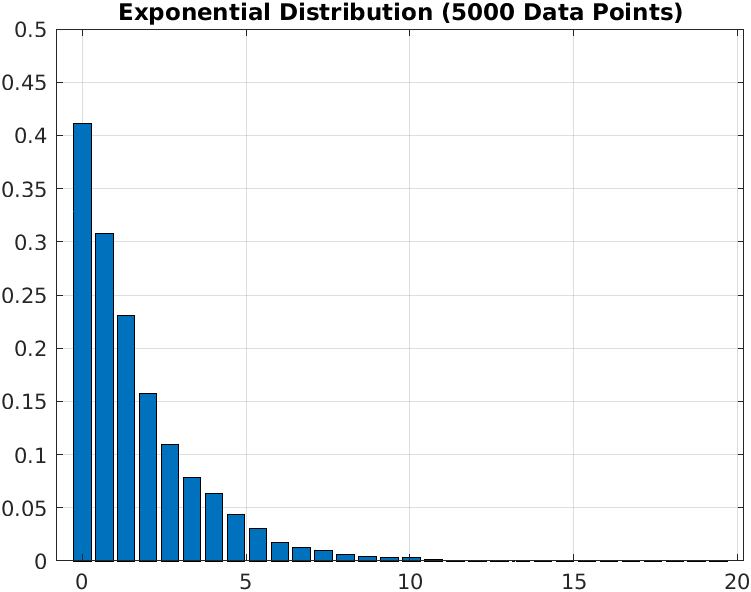
\includegraphics[width=\linewidth]{exp_5k.png}    
    \end{subfigure}
\end{figure}

The Exponential Distribution is a continuous probability distribution that describes the time between events in a Poisson process, where events occur at a constant average rate $\lambda$. It's characterized by a single parameter, the rate parameter $\lambda$, which controls the rate of decay of the exponential curve. The mean of the Exponential Distribution is equal to $1/\lambda$, and the standard deviation is also equal to $1/\lambda$. 

If the shape is considered, then the Exponential Distribution seems to follow a similar shape to the Gamma Distribution after its peak value. And indeed, the Exponential Distribution is a special case of the Gamma Distribution, where the shape parameter $\alpha$ is equal to 1. However, they both have different use cases.

\newpage
\subsection*{Rayleigh Distribution}

\textbf{MATLAB Code:}
\begin{lstlisting}[caption={Rayleigh Distribution},label={Rayleigh}]
>> sigma = 0.1; %Scale Parameter
>> DATA = sigma * randn(1, 5000); %Change value from 5000 to 500 for 500 data points
>> BINS = 30; 
>> [COUNTS,EDGES] = histcounts(DATA,BINS); 
>> Ediff=diff(EDGES); 
>> WIDTH=Ediff(1); 
>> AREA=sum(COUNTS)*WIDTH;
>> figure; bar(EDGES(1:end-1), COUNTS/AREA); 
>> title('Rayleigh Distribution (5000 Data Points)'); grid on;
\end{lstlisting}

\begin{figure}[htbp]
    \begin{subfigure}[b]{0.5\textwidth}
        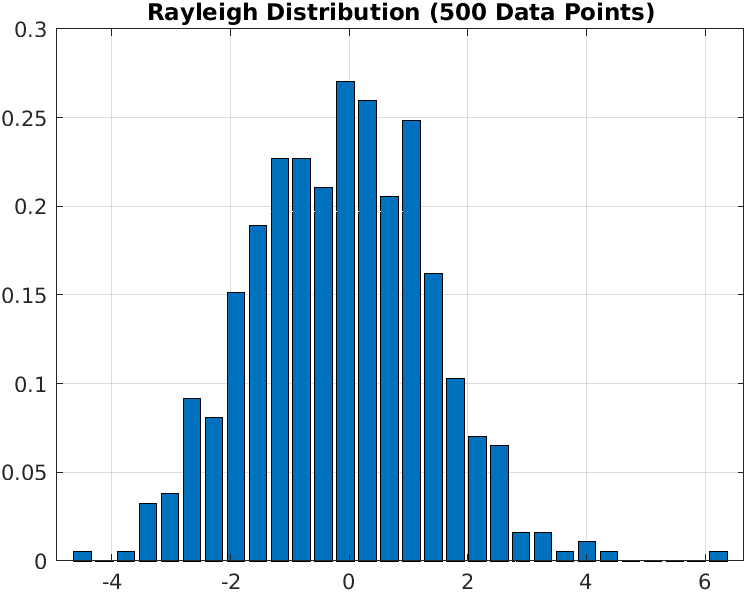
\includegraphics[width=\linewidth]{rayleigh_5.png}
    \end{subfigure}
    \begin{subfigure}[b]{0.5\textwidth}
        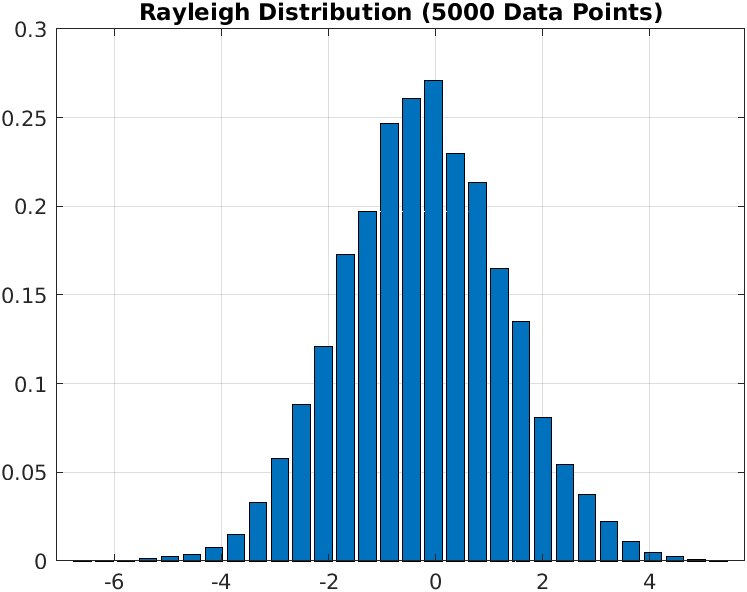
\includegraphics[width=\linewidth]{rayleigh_5k.png}    
    \end{subfigure}
\end{figure}

The Rayleigh Distribution is a continuous probability distribution, characterized by a single parameter $ \sigma $, the scale parameter. It has a slightly right skewed, unimodal curve with a peak, commonly used to model the amplitude of signals in noise. In contrast, it looks more like the Gaussian Distribution, but it's not symmetrical, but its not completely skewed like the Gamma Distribution either.

\end{document}